\chapter{Ergebnisse}

\section{Energie Rekonstruktion mit Hilfe eines Random Forest Regressors}

Um ein Vergleichsergebnis zu erhalten, wird zunächst ein RandomForest Regressor, wie er in \autoref{sec:RF} beschrieben ist, verwendet,
der eine Energieschätzung für jedes Teleskop vornimmt.
Für das Training werden nur Gamma Ereignisse verwendet und somit eine erfolgreiche Signal-Untergrund Trennung vorrausgesetzt.
Es werden jedoch zerstreute und punktgerichtete Gamma Simulationsdaten verwendet, womit das Testen realitätstreuer ist, da in der
Realität die Signal Extraktion nicht zwischen punktgerichteten Photonen und Photonen, die in der Atmosphäre entstehen oder zu der
allgemeinen kosmische Strahlung gehören, unterscheiden kann.

Als Attribute werden die nicht richtungsabhängigen Hillasparameter verwendet, dazu gehören Intensität, Länge, Weite, Schiefe und Weite, sowie
die totale Intensität, die von allen Teleskopen, die das gleiche Ereignis gesehen haben, aufgenommen wird.
Zusätzlich werden die Anzahl der ausgelösten Teleskope, SST, MST und LST als Attribute verwendet, sowie die Identifikationsnummer des
Teleskopes, welche für das LST $1$, für das MST $2$ und für das SST $3$ ist.

Desweiteren werden die skalierte Länge und Weite verwendet, die durch
\begin{equation}
  SW = \frac{w- \langle w \rangle}{\sigma_w}
\end{equation}
und
\begin{equation}
  SL = \frac{l - \langle l \rangle}{\sigma_l}
\end{equation}
definiert sind, wobei der Mittelwert über alle Trainingsdatenwerte genommen wird. Diese Methode nennt sich Scaled Cuts Technik.\cite[104]{HESS}

Der ganze Datensatz besteht aus $\num{3322938}$ Datenpunkten, die durch die \textsc{train\_test\_split}-Funktion der \textsc{sklearn}-Bibliotheke
in einen Trainings und Testdatensatz aufgeteilt wird. Dabei wird mit $\SI{33}{\percent}$ der Daten trainiert und mit $\SI{66}{\percent}$
getestet. Die Aufteilung geschieht jedoch mithilfe der Ereignisnummer, damit bei der Trennung keine Ereignisse getrennt werden.

Bei dem Training werde ein Random Forest verwendet, der eine Maximal Tiefe von $10$ Ebenen besitzt, damit es nicht zum Übertraining
kommt, da der Trainingsdatensatz $\num{1129798}$ Datenpunkte besitzt.
Jeder Baum trainiert mit $\sqrt{N}$ Attributen,wobei $N$ Attribute zur Verfügung stehen, da sonst die Bäume nicht mehr unkorreliert
sind und somit die Ergebnisse der einzelnen Bäume nicht mehr verschieden sind.
Außerdem besteht der Wald aus $100$ Bäumen, wobei dieser Parameter mit einer größeren Rechenleistung vergrößert werden kann, ohne
das es zum Übertraining kommt, was in \autoref{sec:RF} genauer erklärt ist.
Die anderen Hyperparameter sind nicht manuell verändert und somit nutzt der Algorithmus das in \autoref{sec:RF} beschriebene Kriterium der
Varianz Reduktion.
Da die gering gewählte Tiefe ein Übertraining bereits verhindern sollte und das Problem viel Statistik besitzt, werden die Hyperparameter
der minimalen Blatt und Trenngröße auf ihrer Grundeinstellung von $1$ und $2$ gelassen.

\begin{figure}
  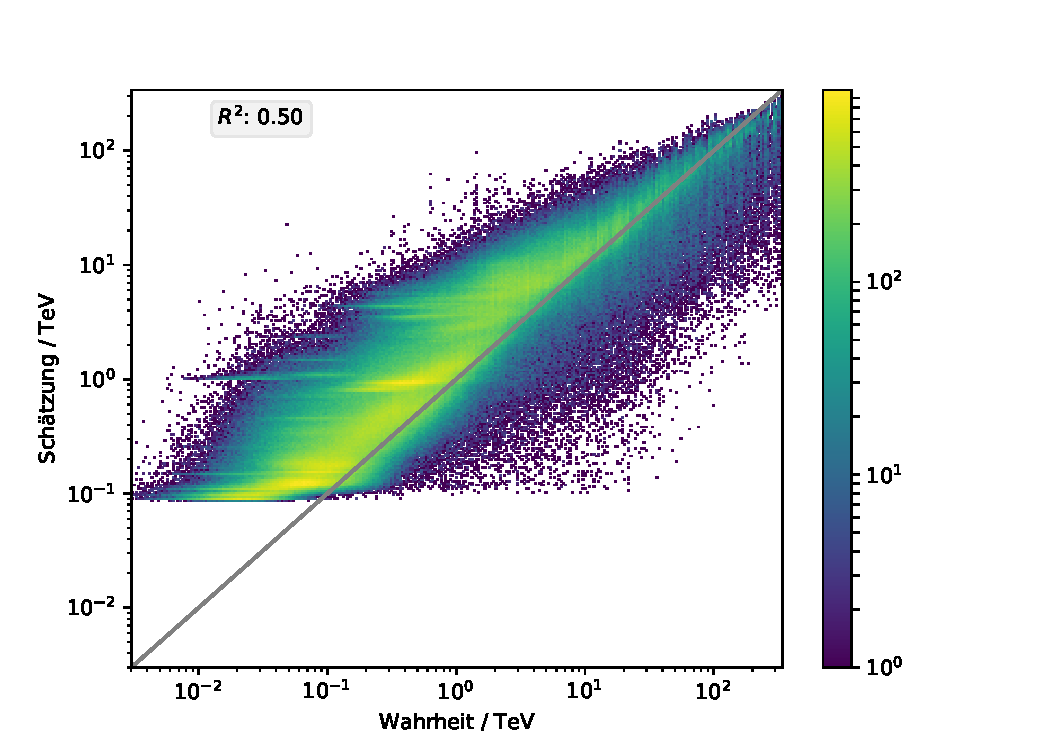
\includegraphics[width=\textwidth]{Plots/RF.pdf}
  \centering
  \caption{In diesem Graph ist die vorhergesagte Energie gegen die Wahrheit aufgetragen, dabei ist eine Streuung mit einer Verzerrung um die
          Diagonale zu erkennen.}
  \label{abb:Energie_RF}
\end{figure}

Dieser trainierte Entscheidungswald wird mit $\num{2193140}$ Datenpunkten getestet und liefert eine Performance, wie sie in \autoref{abb:Energie_RF} zu sehen ist.
Dabei ist eine Überschätzung der Wahrheiten zu beobachten, sowie feine horizontale Linien, die auf eine Korreliertheit der Entscheidungsbäume hindeutet.
Der $R^2$-Wert von $\num{0.50}$ deutet auf eine bessere Beschreibung des Modells als der bloße Mittelwert hin.
Die Korreliertheit und die Verzerrung kann durch eine geeignetere Wahl der Hyperparameter minimiert werden, jedoch ist dies nicht das Ziel dieser
Arbeit.

\begin{figure}
  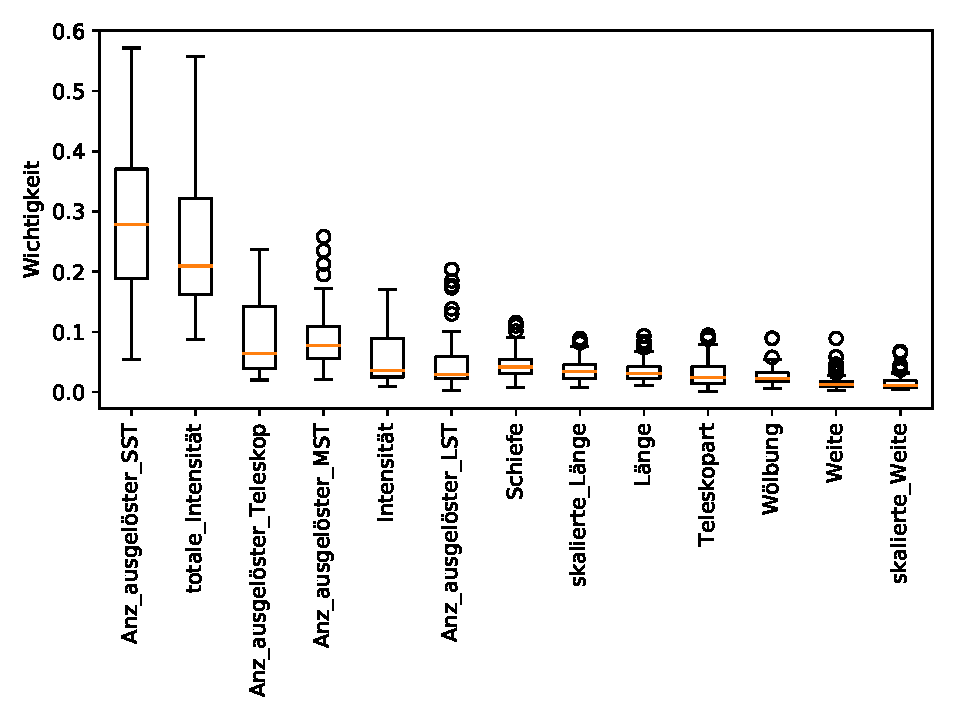
\includegraphics[width=\textwidth]{Plots/feautureimportance_boxplot_firstForest.pdf}
  \centering
  \caption{Darstellung der Wichtigkeit der genutzen Attribute bei der ersten Vorhersage als Kastengrafik. Die Anzahl der ausgelösten SST und die totale Intensität
          stellen die wichtigsten Attribute dar und die Weite trägt kaum zur Schätzung bei.}
  \label{abb:first_FI}
\end{figure}

In \autoref{abb:first_FI} ist die Wichtigkeit der Attribute aufgeführt, wobei zur Darstellung eine Kastengrafik genutzt wird.
Dabei stellt die grüne Linie den Median dar, die Enden des Kastens das $\num{0.25}$- und das $\num{0.75}$-Quartil, die Antennen das $\num{0.125}$- und das
$\num{0.875}$-Quantil und die Punkte Ausreißer die außerhalb des $\num{0.75}$-IQA liegen.
Eventspezifische Attribute wie die Anzahl der ausgelösten Teleskope und die totale Intensität besitzen die größte Wichtigkeit und teleskopspezifische Attribute
wie die Hillasparameter scheinen keinen großen Informationsgewinn zu liefern.
Eine Erklärung liefert die Tatsache, das ein wichtiger Parameter für die Energieschätzung die in dem Schauer deponierte Energie ist und die Hillasparameter im
Gegensatz zu den eventspezifischen Parametern von dem Abstand des Teleskopes zum Schauer abhängen.

\section{Optimierung durch Mittelwerte und geeignete Gewichte}

Die Energieschätzung der einzelnen Teleskope bei einem Ereignis variiert, obwohl sie das gleiche Schauer beobachten.
Dies liegt an dem unterschiedlichen Blickwinkel und Abstand der Teleskope, was dazu führt das jedes Teleskop unterschiedlich viel Information über das
Schauer besitzt.
Es wird angenommen, dass die variierenden Ergebnisse zufällig und nach den Zentralen Grenzwertsatz der Statistik normalverteilt um den
wahren Wert liegen\cite[10]{zufall_Fehler}.
Daher wird als Schätzer des wahren Wertes das arithmetische Mittel und der Median untersucht.
\begin{figure}
  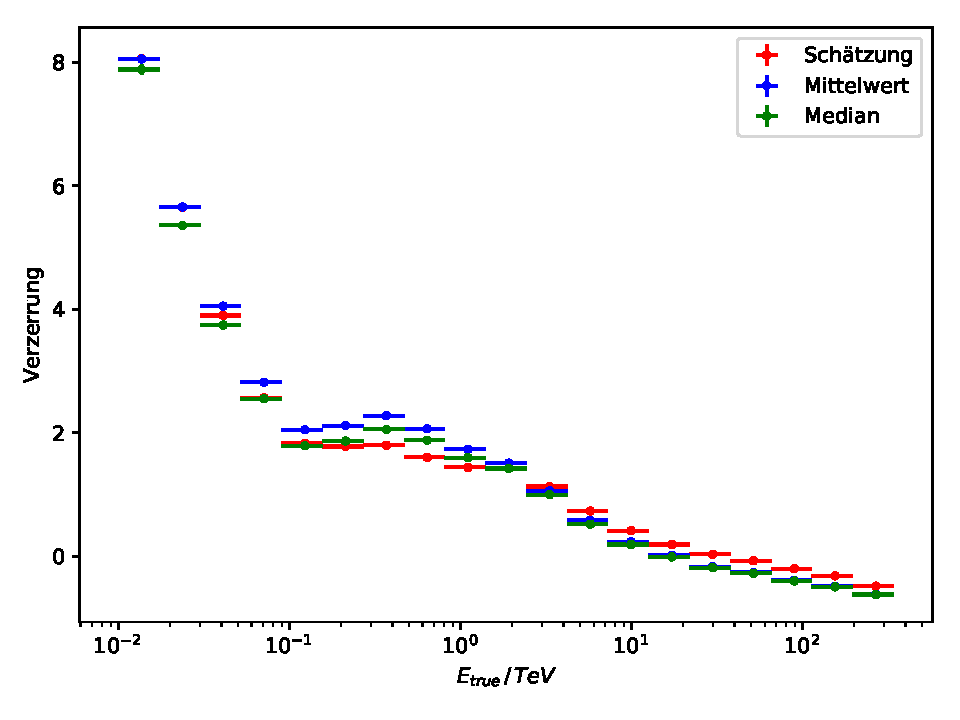
\includegraphics[width=\textwidth]{Plots/RF_mean_bias.pdf}
  \centering
  \caption{Darstellung der Verzerrung für verschiedene Energiebereiche. Es sind die Mittelwerte der relativen Fehler für die erste Vorhersage, die Vorhersage
          nach der Mittelwert Bildung und der Median der Vorhersagen aufgetragen.}
  \label{abb:mean_median_bias}
\end{figure}
\begin{figure}
  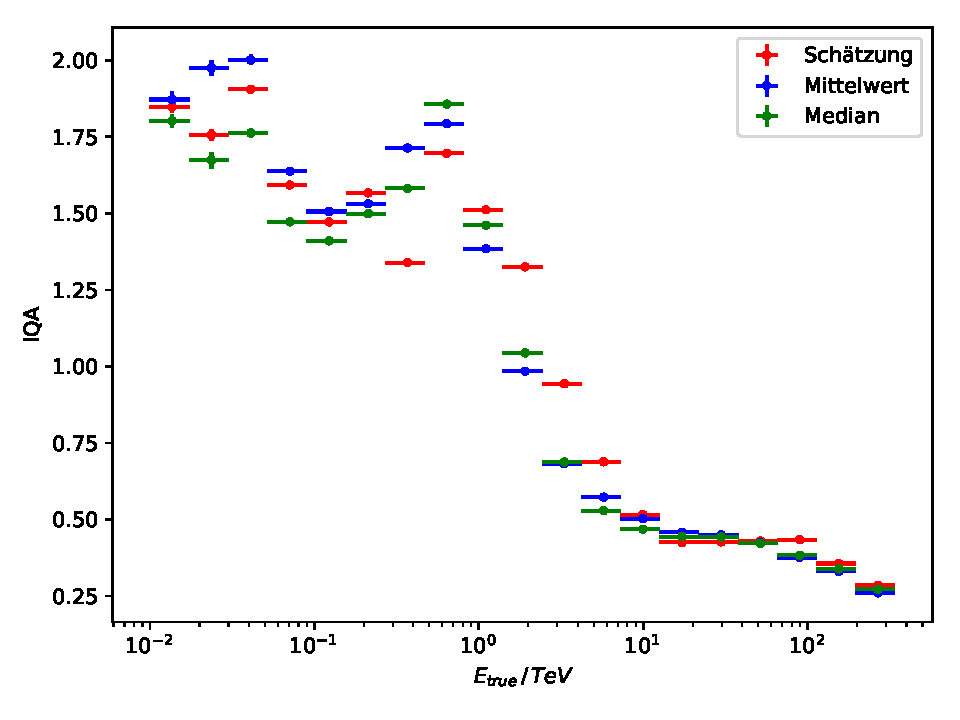
\includegraphics[width=\textwidth]{Plots/RF_mean_resolution.pdf}
  \centering
  \caption{Darstellung des IQA des relativen Fehlers für verschiedene Energiebereiche. Aufgetragen sind die erste Vorhersage, die Vorhersage
          nach der Mittelwert Bildung und der Median der Vorhersagen.}
  \label{abb:mean_median_IQA}
\end{figure}
Die zusammengefassten Schätzungen führen auf die Verzerrungen und IQA's, die in \autoref{abb:mean_median_bias} und \autoref{abb:mean_median_IQA} zusehen sind.
Bei der Bildung des Median ist die erwartete Verbesserung zu beobachten.
Das Schätzen mithilfe des Mittelwerts führt jedoch zu einer Verschlechterung des Ergebnisses.
Bei dem Beobachten von Schauern kann es vorkommen, dass einzelne Teleskope im Gegensatz zu anderen besser positionierten Teleskopen nur einen geringen Teil
des Schauers beobachten und somit wenig Information des Schauers besitzen und eine ganz falsche Vorhersage liefern.
Dies sind meist nur vereinzelte Teleskope und die Mehrheit der Teleskope liegt richtig.
Jedoch führt eine Mittelung dazu, dass diese eine Schätzung den Mittelwert verschlechtert.
Das die Verzerrung nur in der Mitte des Energiebereiches größer ist, liegt daran, dass der genannte Effekt bei geringen Energien und somit kleinen Schauern
nicht so groß ist, da dort die Kamerabilder grundsätzlich wenig Information beinhalten.
Und bei großen Energien sind die Scheuer meistens groß genug, dass genug Teleskope ausreichend Information beinhalten.

Dass Telekope mit schwachem Kamerabild das Zusammengefasste Ergebnis verschlechtern, kann nicht auftreten, wenn der Median berechnet wird.
Dadurch führt der Median auf eine bessere Schätzung als die Mittelwert Bildung und normalverteilten Ergebnisse liefern zusammengefasst ein besseres Ergebnis,
was in \autoref{abb:mean_median_bias} und \autoref{abb:mean_median_IQA} zu erkennen ist.

Eine weitere Möglichkeit um das Problem zu beheben, dass nicht alle Telskope das Schauer gleich gut sehen, ist das Mitteln mit einem Gewicht, welches die
Sichtbarkeit des Schauers beschreibt.
Die beobachtete Intensität ist zum Beispiel ein Indiz auf den gesehenen Anteil des Schauers, wobei eine hohe
beobachtete Intensität eine gute Sichtbarkeit bedeutet und somit die Intensität direkt als Gewicht verwendet wird.

Zum Anderen besitzten die in \autoref{sec:CTA} beschriebenen Teleskope eine energieabhängige Sensitivität, wobei
es einen Energiebereich gibt bei dem eine volle Sensitivität herrscht und ein Bereich indem eine Teilsensitivität
herrscht.
Das LST besitzt eine Teilsensitivität bei $\SI{20}{\giga\eV}-\SI{3}{\tera\eV}$ und eine volle Sensitivität bei
$\SI{20}{\giga\eV}-\SI{150}{\giga\eV}$.
Das MST ist teilsensitiv bei $\SI{80}{\giga\eV}-\SI{50}{\tera\eV}$ und vollsensitiv bei $\SI{150}{\giga\eV}-\SI{5}{\tera\eV}$
und das LST hat seine Teilsensitivität bei Energien zwischen $\SI{1}{\tera\eV}-\SI{300}{\tera\eV}$ und seine
Hauptsensitivität bei $\SI{5}{\tera\eV}-\SI{300}{\tera\eV}$.\cite{CTA_tec}
Wenn die geschätzte Energie im vollsensitiven Bereich liegt, wird ein Gewicht von $2$ angelegt, wenn sie im
teilsensitiven Bereich liegt ein Gewicht von $1$ und wenn die Energie in keinem Sensitivitätsbereich liegt
wird ein Gewicht von $0.1$ angelegt.

\begin{figure}
  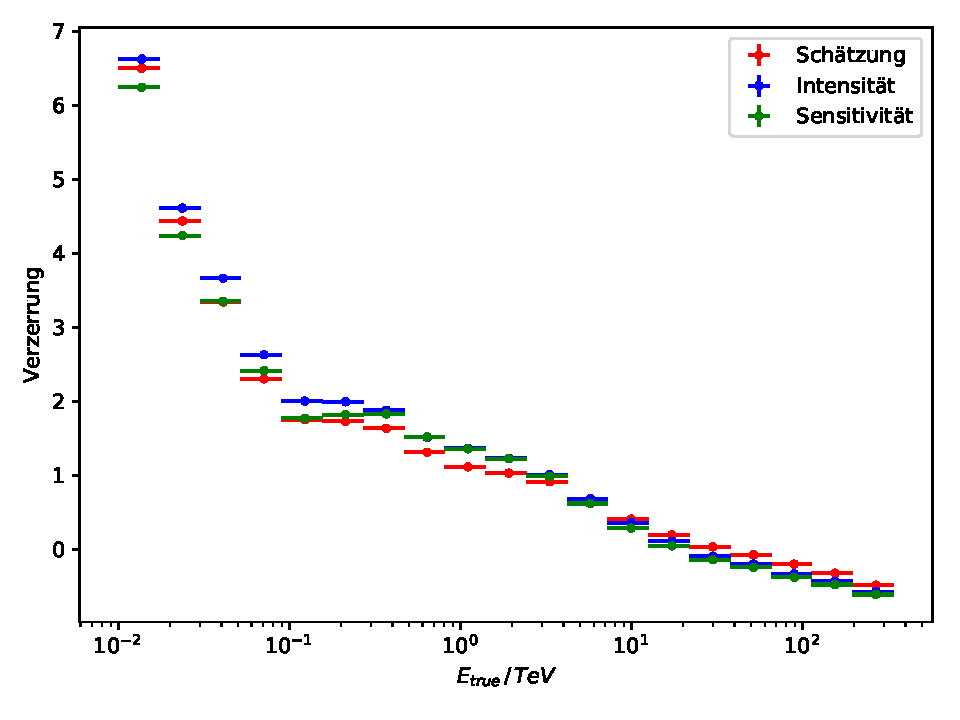
\includegraphics[width=\textwidth]{Plots/RF_weights_bias.pdf}
  \centering
  \caption{Darstellung der Verzerrung für die erste Vorhersage und für eine gewichtete Mittelung mit der Intensität
            oder der Sensitivität als Gewicht.}
  \label{abb:w_bias}
\end{figure}
\begin{figure}
  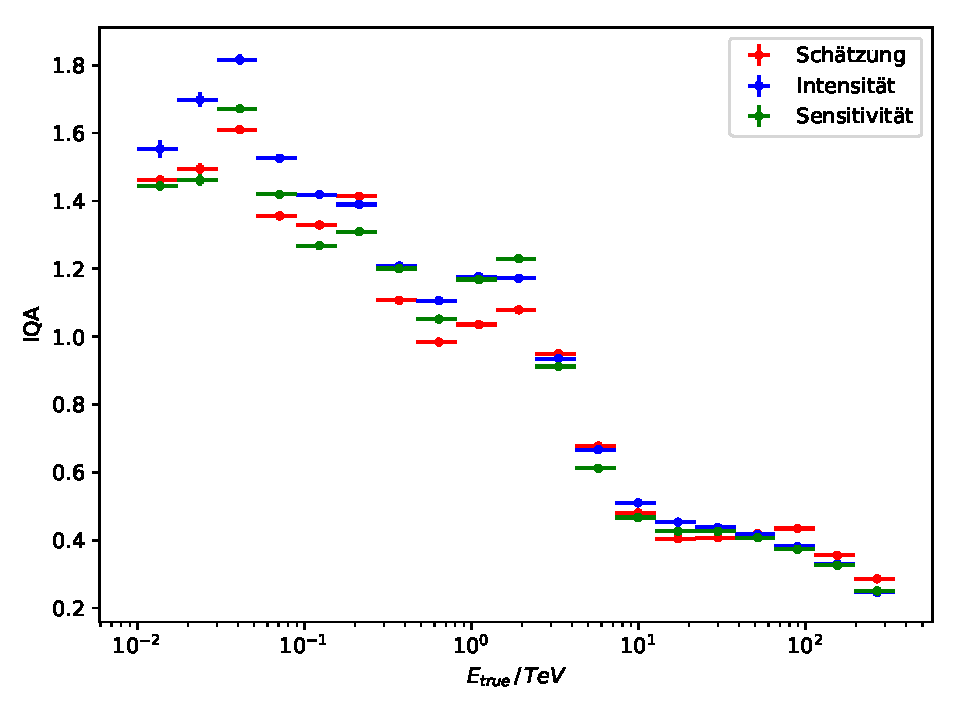
\includegraphics[width=\textwidth]{Plots/RF_weights_resolution.pdf}
  \centering
  \caption{Auftragen des IQA des relativen Fehlers für verschiedene Energiebereiche, jeweils für die erste Vorhersage und
            für die mit der Intensität oder der Sensitivität gewichtet gemittelten Vorhersage.}
  \label{abb:w_IQA}
\end{figure}
Das Gewichten führt auf eine Energieschätzung, die in \autoref{abb:w_bias} und \autoref{abb:w_IQA} zu sehen ist.
In beiden Abbildungen ist keine Verbesserung des Schätzers im Vergleich zu einer ungemittelten Vorhersage zu erkennen, was darauf schließen lässt,
dass entweder die meisten Fehlschätzungen nicht durch die schlechte Sicht auf das Schauer entstehen, sondern andere Gründe haben oder die
Gewichte sind nicht gut genug für den Ausgleich geeignet.

%Einfacher Mittelwert über gleiches Event; Nutzung von unterschiedlichen Gewichten;

\section{Verschachtelung von Regressionsverfahren}

Schon die Wichtigkeit der eventspezifischen Attribute in \autoref{abb:first_FI} deutet darauf hin, dass in der zusammengefassten Attribute eines Ereignisses
mehr Information steckt, als in den teleskopspezifischen Attributen.
Daher wird nach der ersten Schätzung ein zweiter Random Forest trainiert, der nun Schätzungen für jedes Event abgibt und dem eventspezifische Attribute
übergeben werden.
Zu den Attributen gehören die Anzahl der ausgelösten Telskope, sowie SST, MST und LST, die totale Intensität, die gemittelte Schätzung des ersten Waldes,
die Mittelwerte und Standardabweichungen der skalierten Größen und die Mittelwerte, Standardabweichungen, Maximal- und Minimalwerte der Schätzungen von den
SST, MST oder LST.

\begin{figure}
  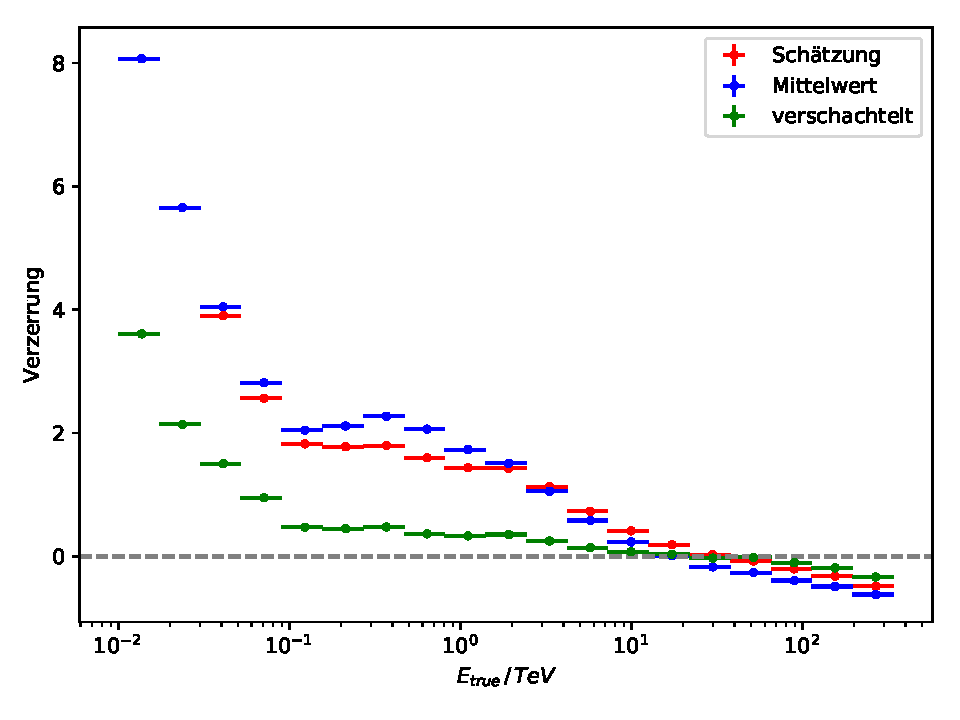
\includegraphics[width=\textwidth]{Plots/RF_nested_bias.pdf}
  \centering
  \caption{Abbildung der Verzerrung nach einer Verschachtelung von zwei Random Forests. Es ist eine deutliche Verbesserung gegenüber der ersten Schätzungen
            zu erkennen.}
  \label{abb:nest_bias}
\end{figure}
\begin{figure}
  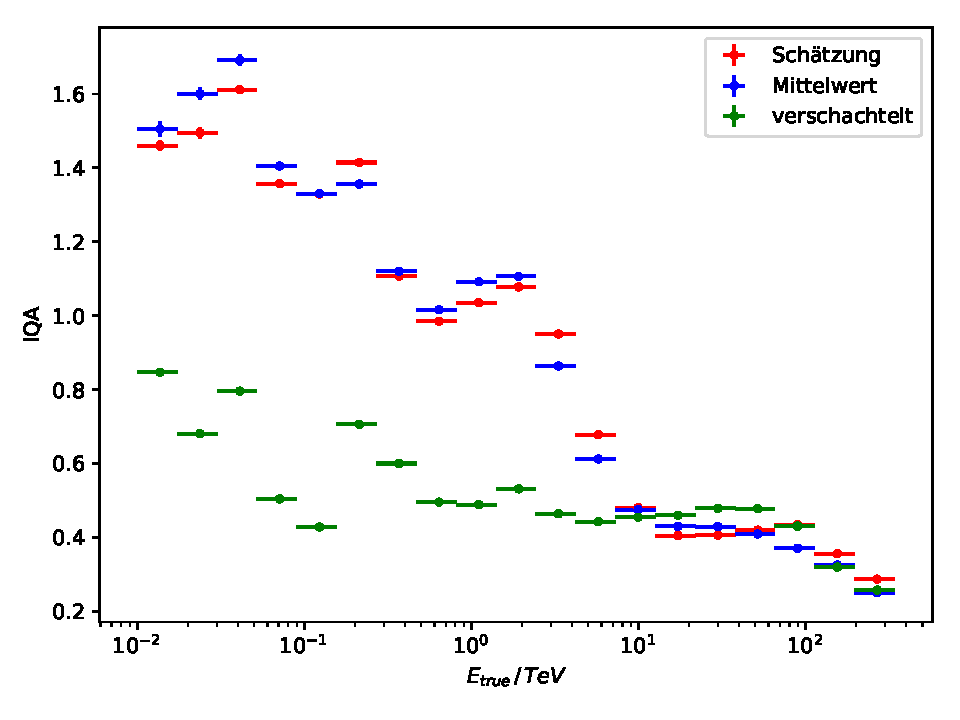
\includegraphics[width=\textwidth]{Plots/RF_nested_resolution.pdf}
  \centering
  \caption{Abbildung des IQA für den zweiten Random Forest. Die Verschachtelung führt auf eine starke Verringerung des IQA bei niedrigen Energien.}
  \label{abb:nest_IQA}
\end{figure}
Der Random Forest wird mit $\num{498081}$ Ereignissen trainiert und mit genauso vielen getestet. Die Performance des zweiten Schätzers ist in \autoref{abb:nest_bias}
und \autoref{abb:nest_IQA} zu sehen.
Die Verschachtelung der Entscheidungswälder führt auf eine verbesserte Performance sowohl bei der Verzerrung als auch bei dem IQA, wodurch ein Übertraining
durch den zweiten Wald ausgeschlossen werden kann.
%Einmal Verschachteln ; Mehrmals Verschafteln gegen die Laufzeit

\section{Transformation der Energie}
